\section{Implementation}
\label{sec:implementation}

\begin{frame}[c]{PyBrain's Architecture for a RL Problem}
\begin{figure}[t!]
	\centering
	\begin{tikzpicture}[node distance = 6em, auto, thick]
		\node (rect) at (0,0) [draw,thick,minimum width=8cm,minimum height=6cm] (Experiment) {};
		\node (rect) at (0,1.4) [draw,thick,minimum width=6cm,minimum height=2cm] (Task) {};
		\node (rect) at (0,1.4) [draw,thick,minimum width=3cm,minimum height=1cm] (Environment) {\texttt{Environment}};
		\node (rect) at (0,-1.4) [draw,thick,minimum width=6cm,minimum height=2cm] (Agent) {};
		\node (rect) at (-1.9,-1.4) [draw,thick,minimum width=1.6cm,minimum height=1cm] (Critic) {\texttt{Critic}};
		\node (rect) at (1.9,-1.4) [draw,thick,minimum width=1.6cm,minimum height=1cm] (Learner) {\texttt{Learner}};
		\node (rect) at (0,-1.4) [draw,thick,minimum width=1.6cm,minimum height=1cm] (Actor) {\texttt{Actor}};
		
		\draw (-2.8,3.3) node {\texttt{Experiment}};
		\draw (-2.4,2.7) node {\texttt{Task}};
		\draw (0.8,0) node {\texttt{Action}};
		\draw (-2.25,1.7) node {\texttt{State}};	
		\draw (2.7,0) node {\texttt{Reward}};
		\draw (-2.4,-2.7) node {\texttt{Agent}};
	
		\path [line] (Task.180) --++ (-0.5cm,0cm) |- node [near start]{\texttt{Observation}} (Agent.180);
		\path [line] (Task.0) --++ (+0.5cm,0cm) |- (Agent.0);
		\draw[line] (Environment.180) -- (Task.180);
		\draw[line] (Agent.90) -- (Task.270); 
	\end{tikzpicture}
\end{figure}	
\end{frame}

\begin{frame}[c]{Agent-Environment Interaction in C++}
	\begin{block}{Adapting PyBrain's Architecture}
		\begin{enumerate}
			\item Defined standard interfaces via pure abstract classes
			\item Achieved modularity via polymorphic composition
		\end{enumerate}
	\end{block}
	
	\begin{figure}[h]
		\centering
		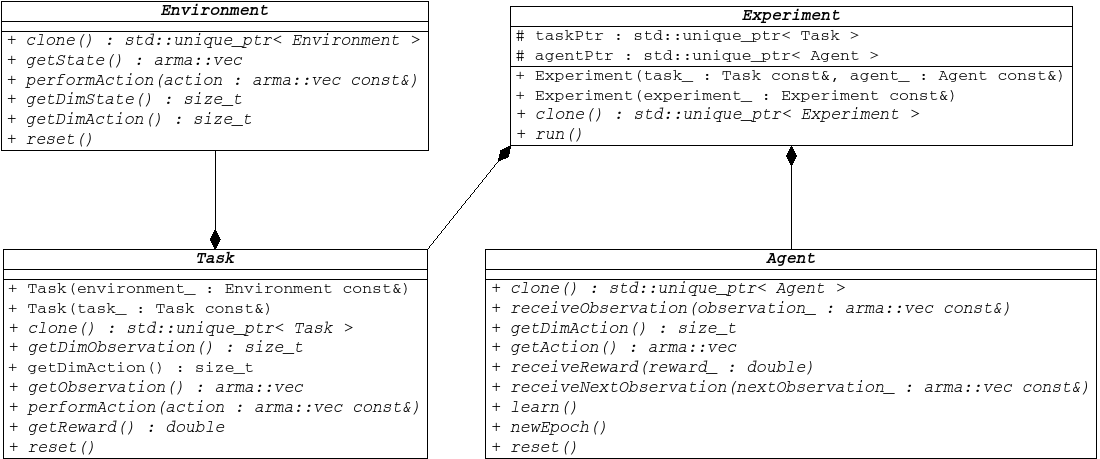
\includegraphics[width=1.0\framewidth]{Images/AgentEnvironmentInteractionReduced}
	\end{figure}
\end{frame}

\begin{frame}[c]{Agent's Architecture in C++}
	\begin{figure}[h]
		\centering
		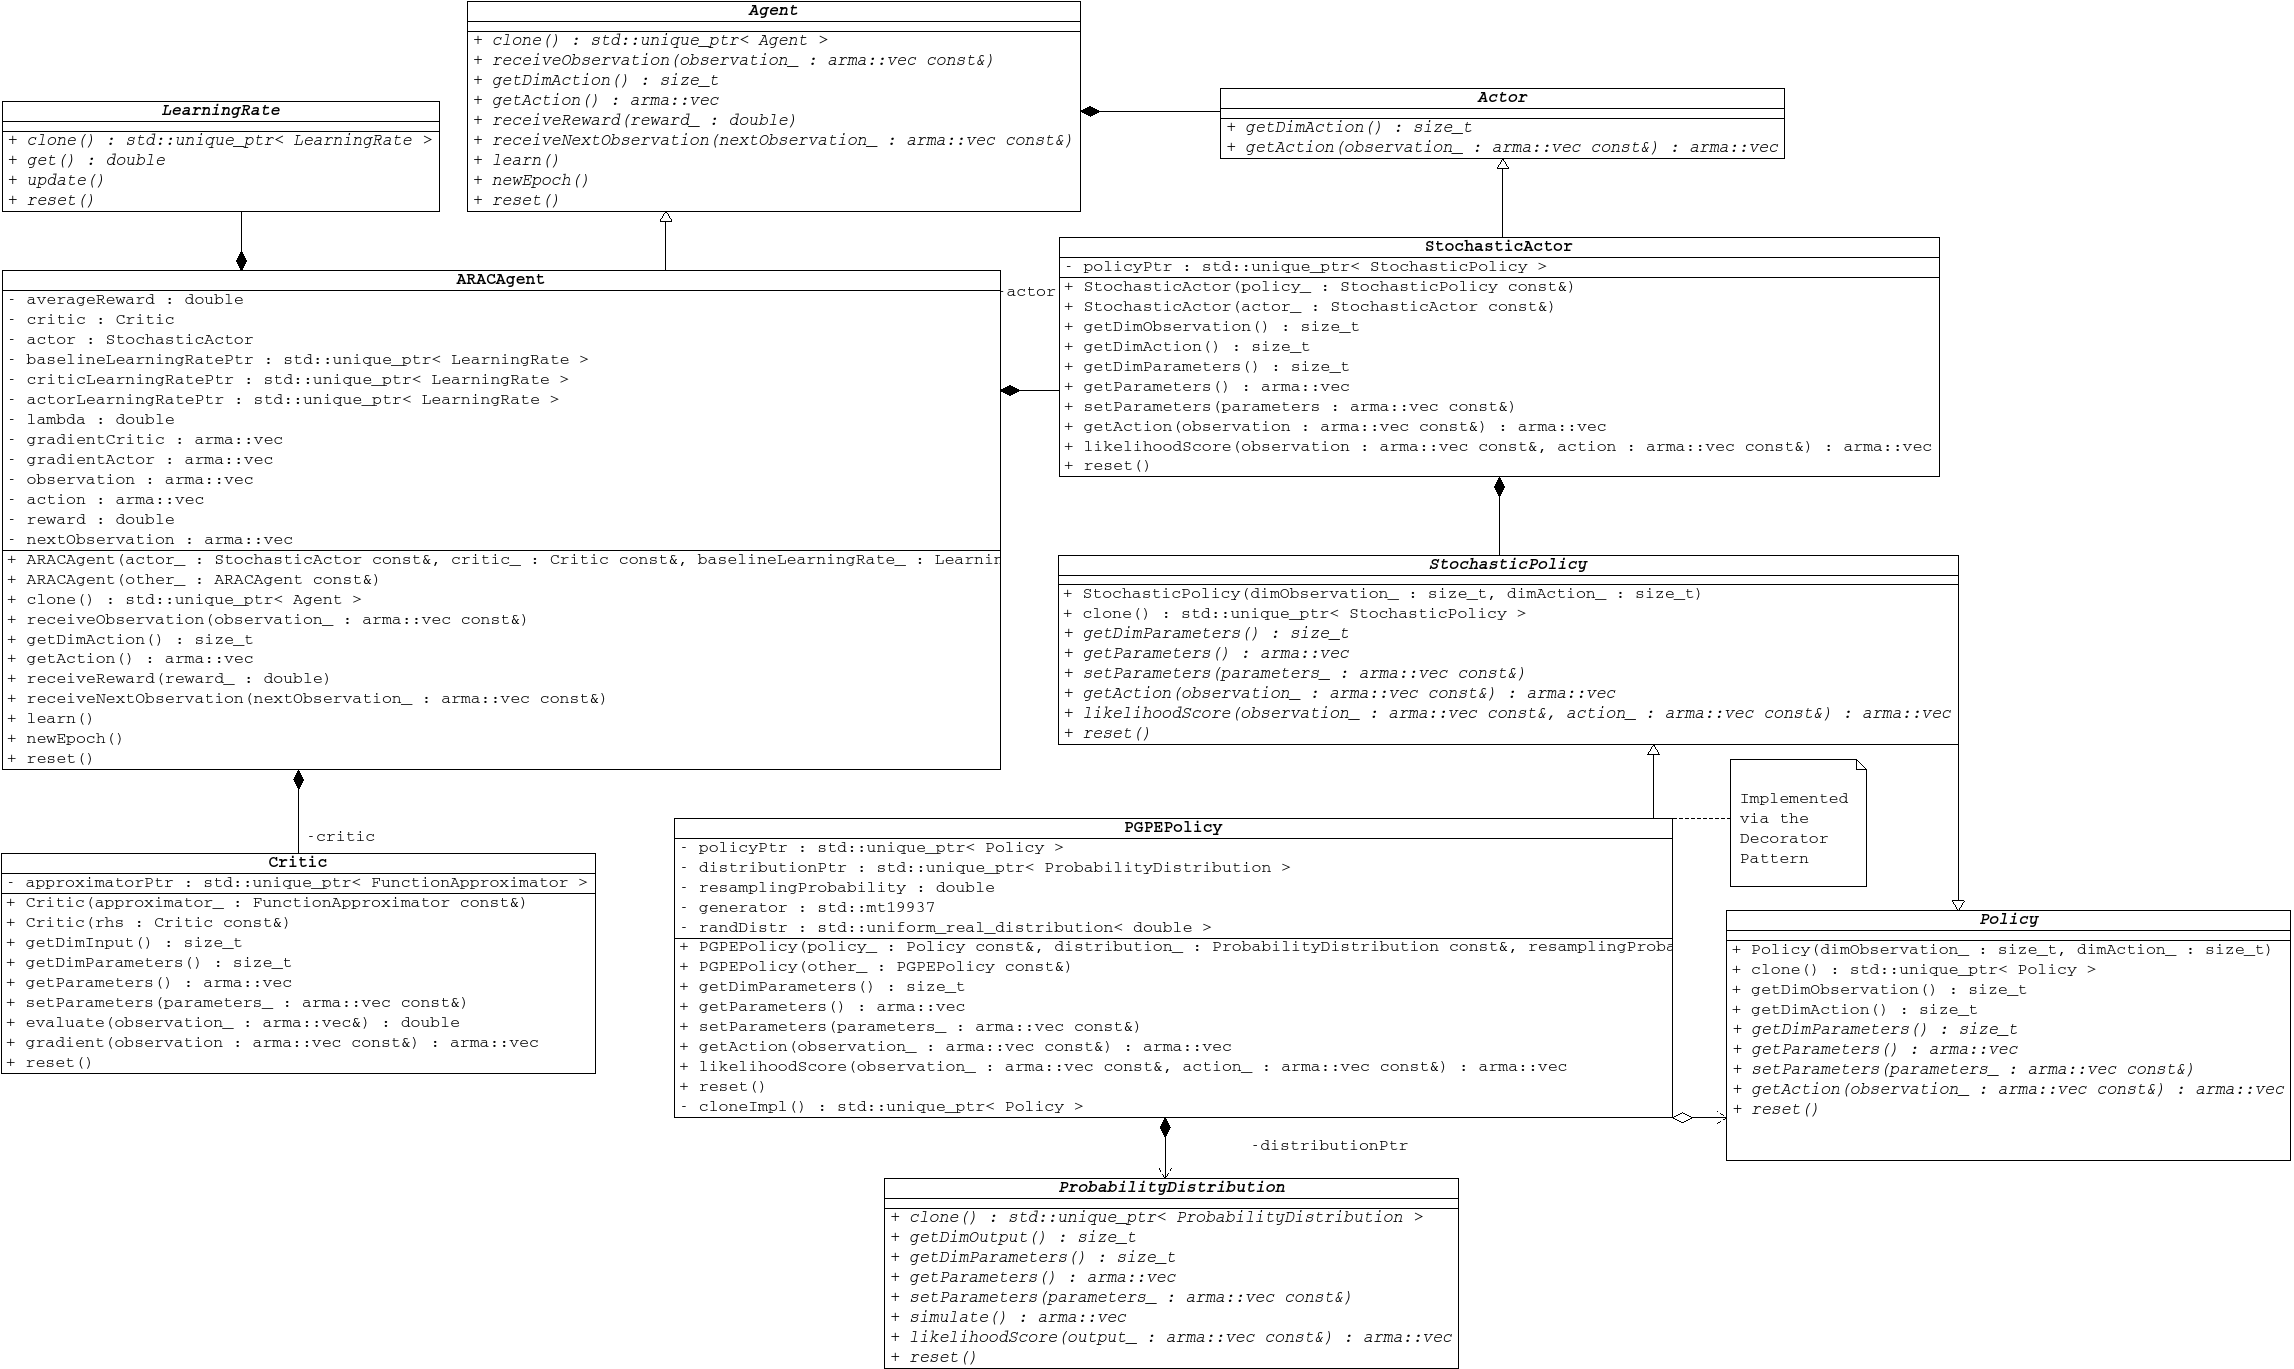
\includegraphics[width=1.0\framewidth]{Images/agent_reduced}
	\end{figure}
\end{frame}

\begin{frame}[c]{Execution Pipeline}
	\begin{block}{\texttt{experiment\_launcher.py}}
		\begin{enumerate}
			\item Program execution is handled by a Python script
			\item Responsible for analyzing the output of the C++ engine
		\end{enumerate}
	\end{block}

	\begin{figure}
		\centering
		\resizebox{\framewidth}{!}{%
		\begin{tikzpicture}[node distance = 6em, auto, thick]
			\node (rect) at (-9.5,-2) [DimGray,draw,thick,minimum width=3cm,minimum height=3cm] (generate_synthetic_series) {};
			\node (rect) at (0,0) [DimGray,draw,thick,minimum width=15cm,minimum height=10cm] (experiment_launcher) {};
			\node (rect) at (+9,-2) [IndianRed,draw,thick,minimum width=2cm,minimum height=3cm] (convergence) {};
			\node (rect) at (+9,+2) [IndianRed,draw,thick,minimum width=2cm,minimum height=3cm] (performance) {};
			\node (rect) at (-6,2) [IndianRed,draw,thick,minimum width=2cm,minimum height=3cm] (input) {};
			\node (rect) at (-6,-2) [IndianRed,draw,thick,minimum width=2cm,minimum height=3cm] (synthetic) {};
			\node (rect) at (-2,0) [SteelBlue, draw,thick,minimum width=4cm,minimum height=8cm] (main_thesis) {};
			\node (rect) at (2,2) [IndianRed,draw,thick,minimum width=2cm,minimum height=3cm] (output) {};
			\node (rect) at (2,-2) [IndianRed,draw,thick,minimum width=2cm,minimum height=3cm] (debug) {};
			\node (rect) at (5.5,0) [DimGray,draw,thick,minimum width=3cm,minimum height=3cm] (postprocessing) {};
			
			\draw (0,5.5) node {\lstinline{experiment_launcher.py}};
			\draw (-9.5,0) node {\lstinline{generate_synthetic_series.py}};
			\draw (-6,-4) node {\lstinline{synthetic.csv}};
			\draw (-7.8,4) node {\lstinline{Single_Synth_RN_P0_F0_S0_N5.pot}};	
			\draw (5.5,2) node {\lstinline{postprocessing.py}};
			\draw (2,4) node {\lstinline{output.csv}};
			\draw (2,-4) node {\lstinline{debug.csv}};
			\draw (9.5,4) node {\lstinline{performance.csv}};
			\draw (9.5,-4) node {\lstinline{convergence.csv}};
			\draw (-2,0) node {\lstinline{main_thesis}};	
		
			\draw[line] (generate_synthetic_series.0) -- (synthetic.180);
			\draw[line] (debug.0) -- (postprocessing.180);
			\draw[line] (output.0) -- (postprocessing.180);
			\draw[line] (postprocessing.0) -- (performance.180);
			\draw[line] (postprocessing.0) -- (convergence.180);
			\draw[line] (input.0) -- (main_thesis.135);
			\draw[line] (synthetic.0) -- (main_thesis.225);
			\draw[line] (main_thesis.45) -- (output.180);
			\draw[line] (main_thesis.315) -- (debug.180);
		\end{tikzpicture}}
	\end{figure}
\end{frame}